In the following figures, the green highlighted values indicate the best achieving evaluation score values (1h or 3h files), for the corresponding clustering method. Furthermore, the dark green highlighted values also accentuate the overall best scoring values over all datasets (1h and 3h files).


\begin{figure}[H]
  \centering
  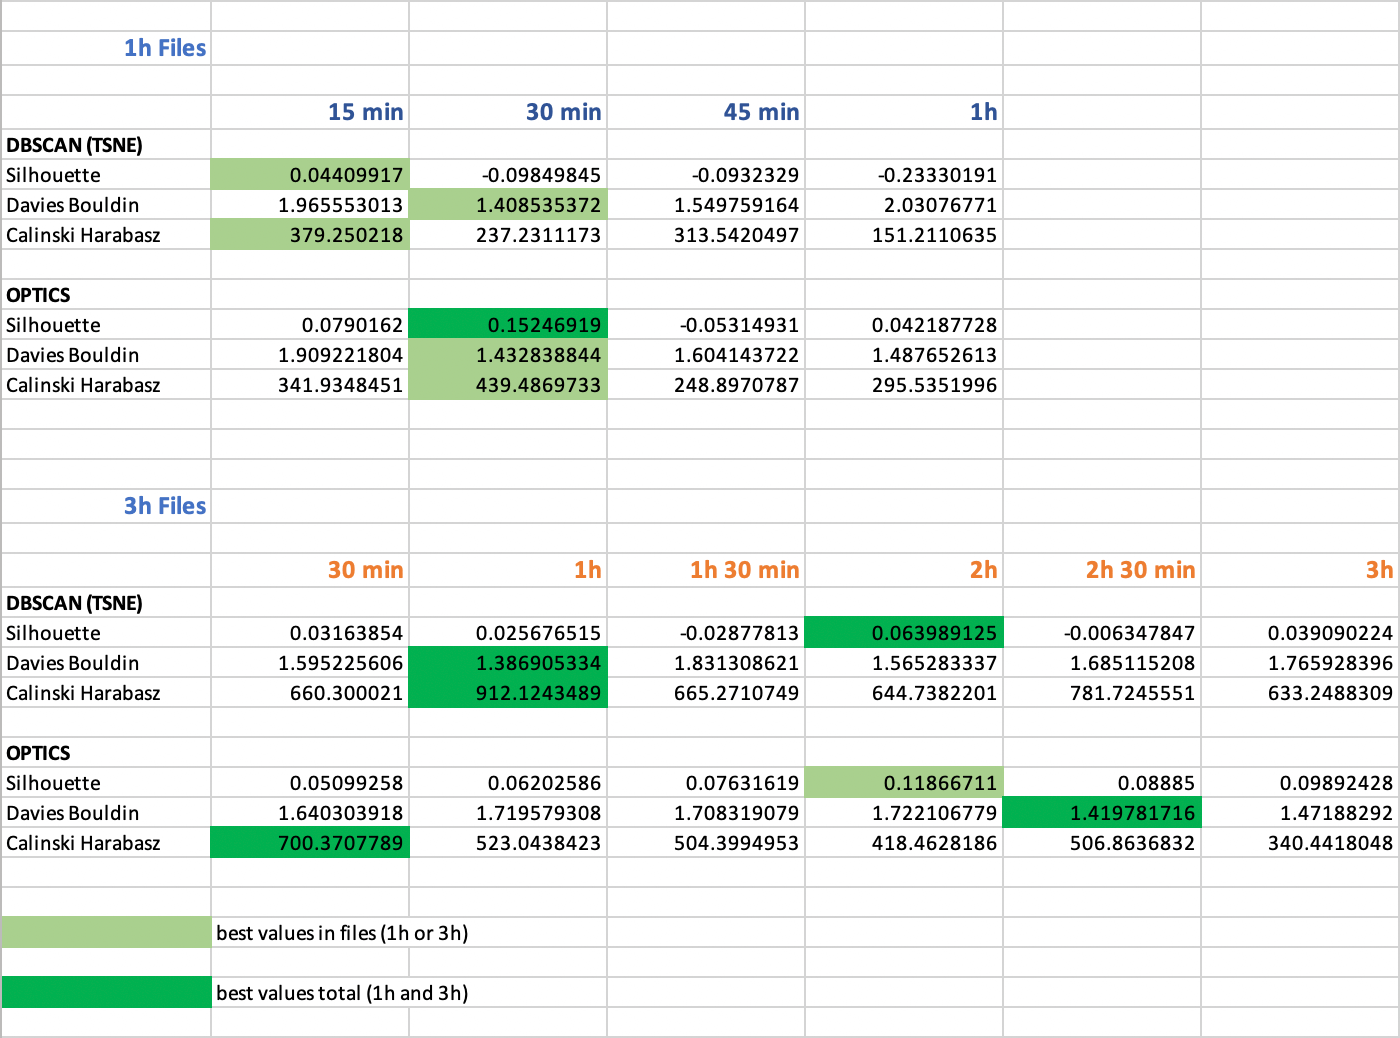
\includegraphics[width=0.8\textwidth]{./images/clusteringResults/clusteringResults1.png}
  \caption{Evaluation scores comparison from the \textbf{first run} of t-SNE and clustering with a \textbf{learning rate of 20}.}
  \label{figure:clusteringResults1}
\end{figure}

\begin{figure}[H]
  \centering
  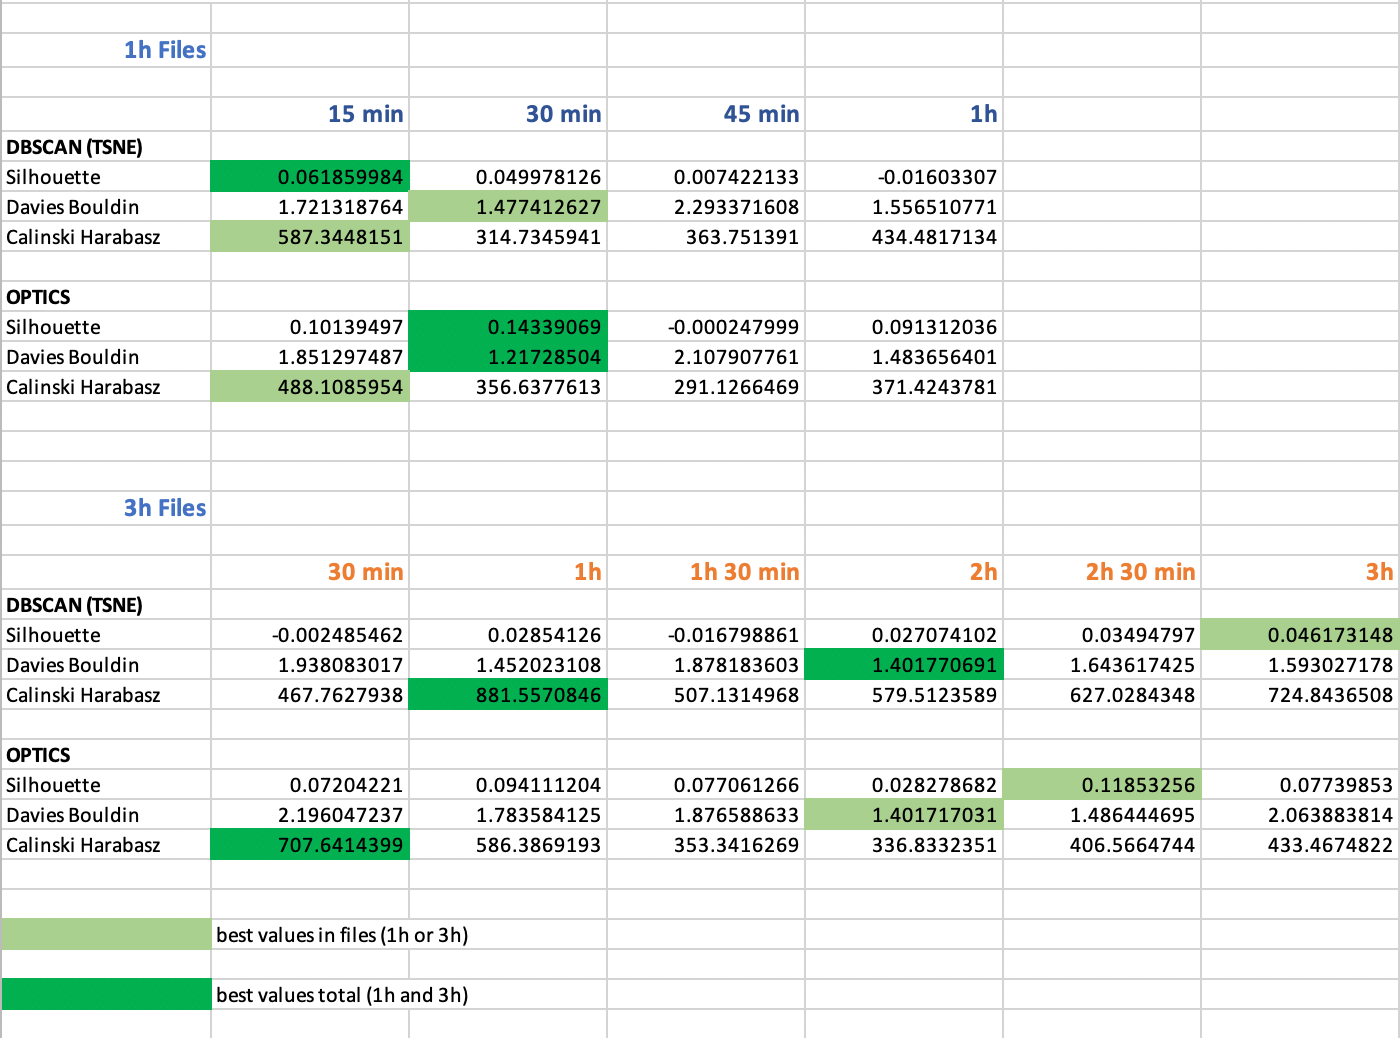
\includegraphics[width=0.8\textwidth]{./images/clusteringResults/clusteringResults2.png}
  \caption{Evaluation scores comparison from the \textbf{second run} of t-SNE and clustering with a \textbf{learning rate of 20}.}
  \label{figure:clusteringResults2}
\end{figure}


\begin{figure}[H]
  \centering
  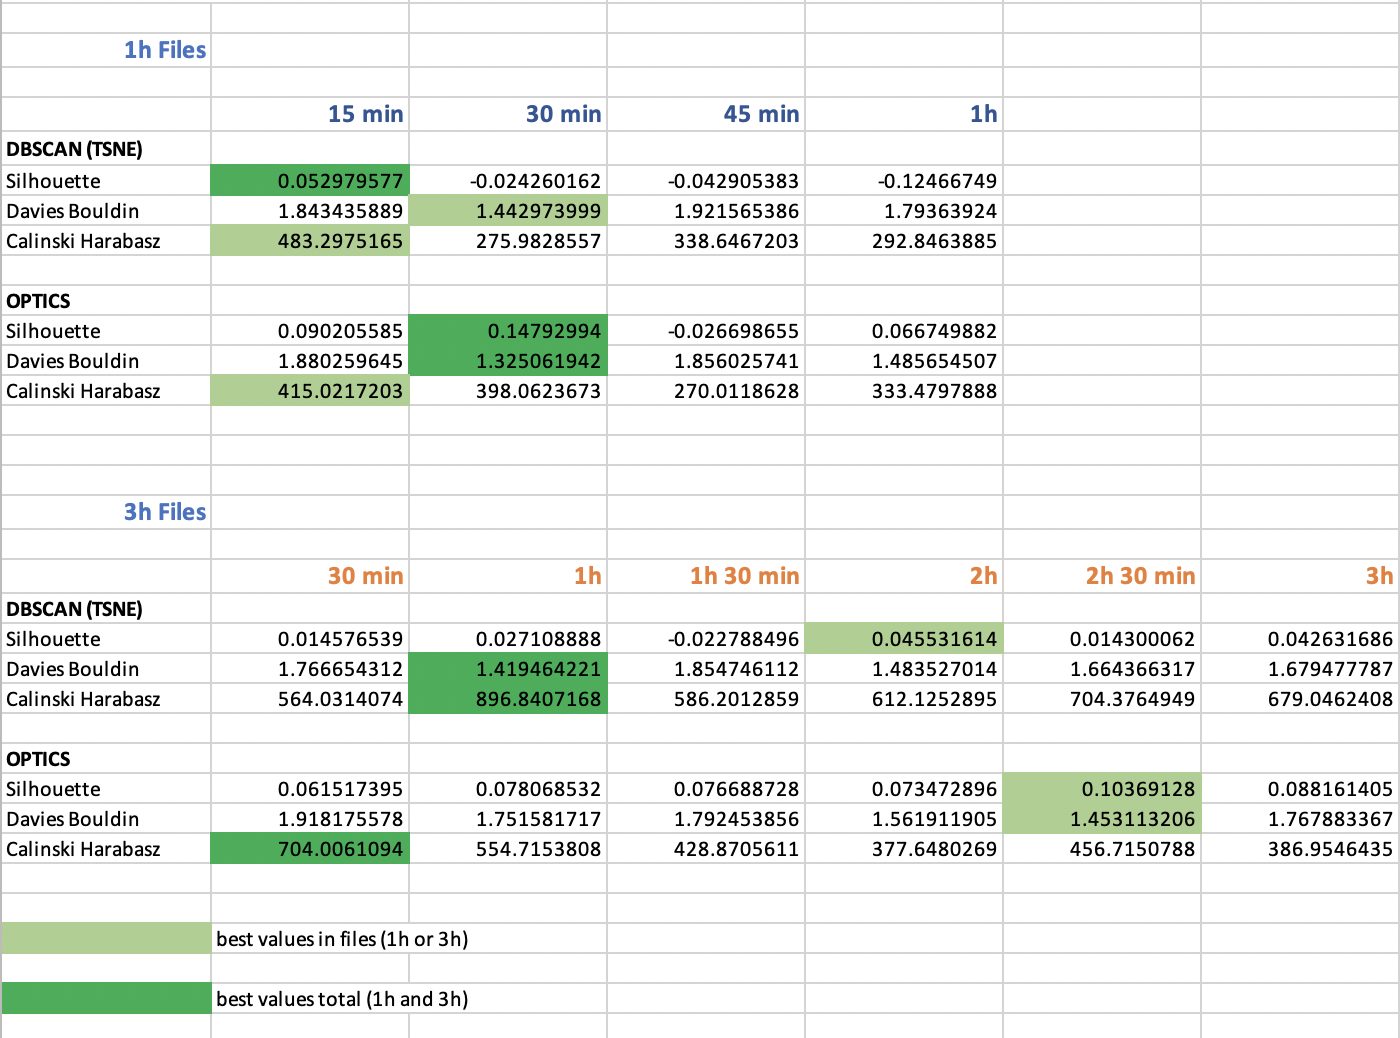
\includegraphics[width=0.8\textwidth]{./images/clusteringResults/clusteringResults3.png}
  \caption{Evaluation scores comparison averaged from \textbf{figures \ref{figure:clusteringResults1} and \ref{figure:clusteringResults2}}.}
  \label{figure:clusteringResults3}
\end{figure}

\begin{figure}[H]
  \centering
  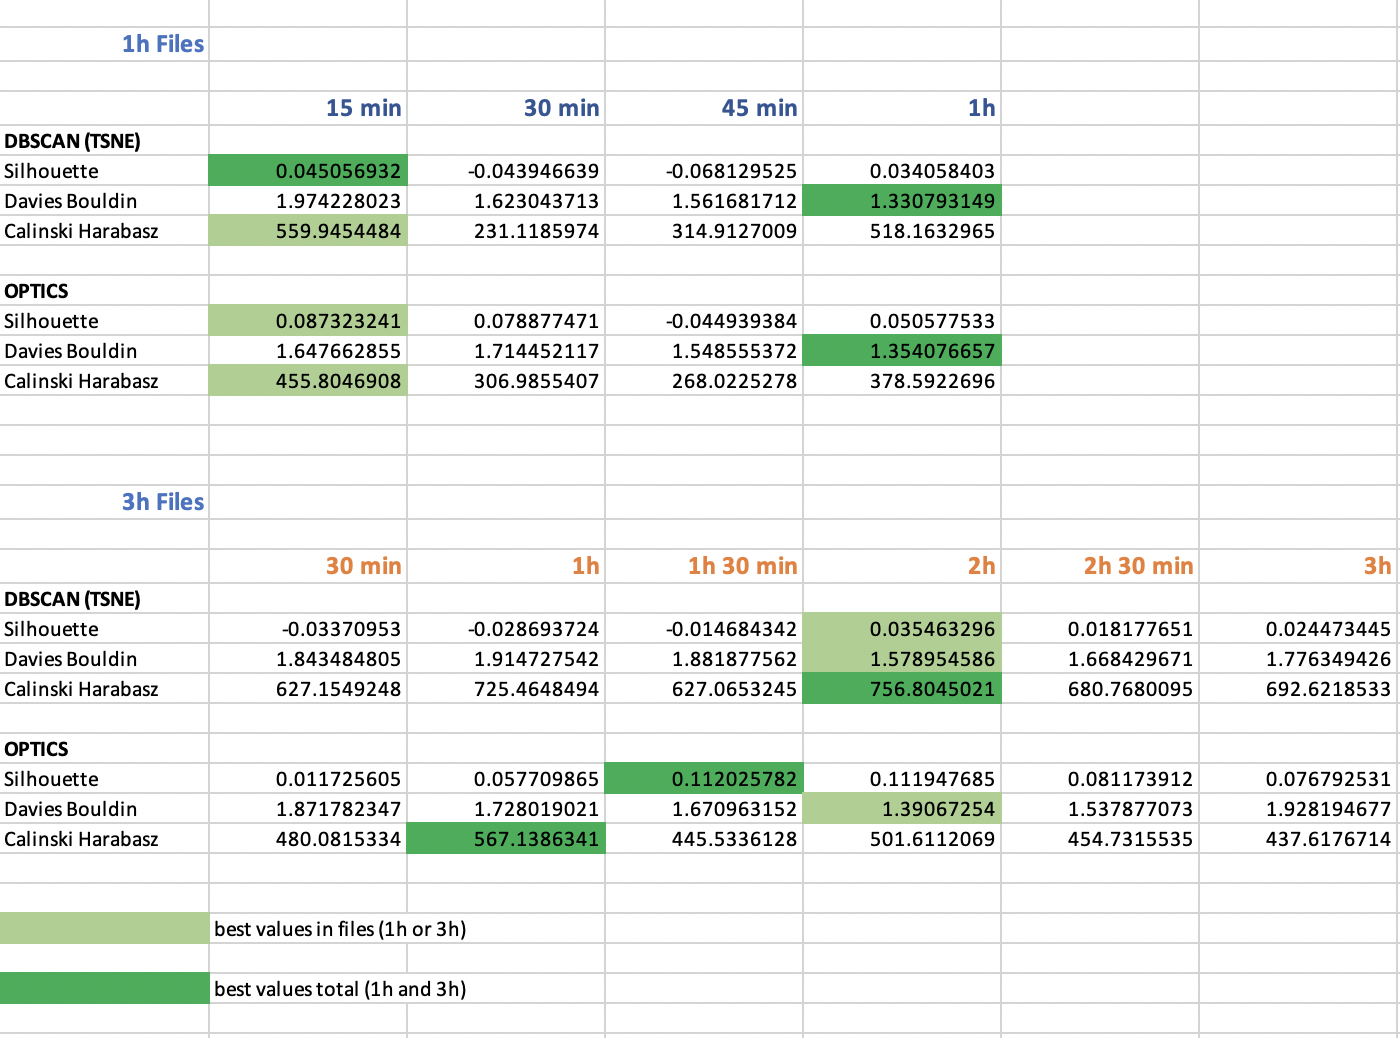
\includegraphics[width=0.8\textwidth]{./images/clusteringResults/clusteringResults4.png}
  \caption{Evaluation scores comparison \textbf{averaged} from \textbf{2 runs} of t-SNE and clustering with a \textbf{learning rate of 20}.}
  \label{figure:clusteringResults4}
\end{figure}

\begin{figure}[H]
  \centering
  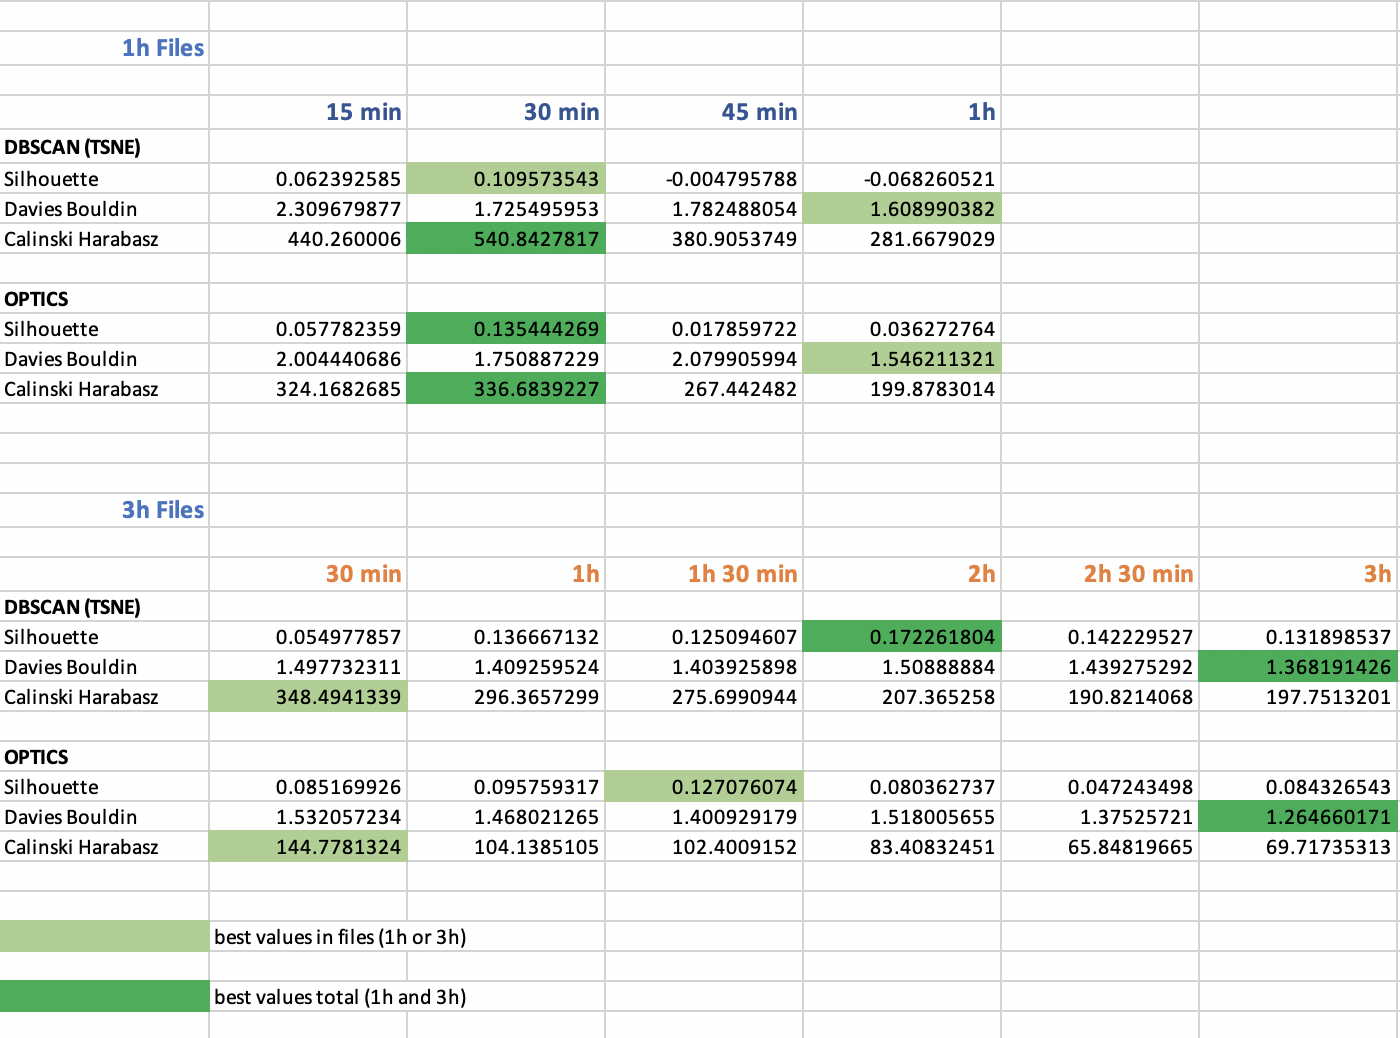
\includegraphics[width=0.8\textwidth]{./images/clusteringResults/clusteringResults5.png}
  \caption{Evaluation scores comparison \textbf{averaged} from \textbf{2 runs} of t-SNE and clustering with a \textbf{learning rate of 800}.}
  \label{figure:clusteringResults5}
\end{figure}

\begin{figure}[H]
  \centering
  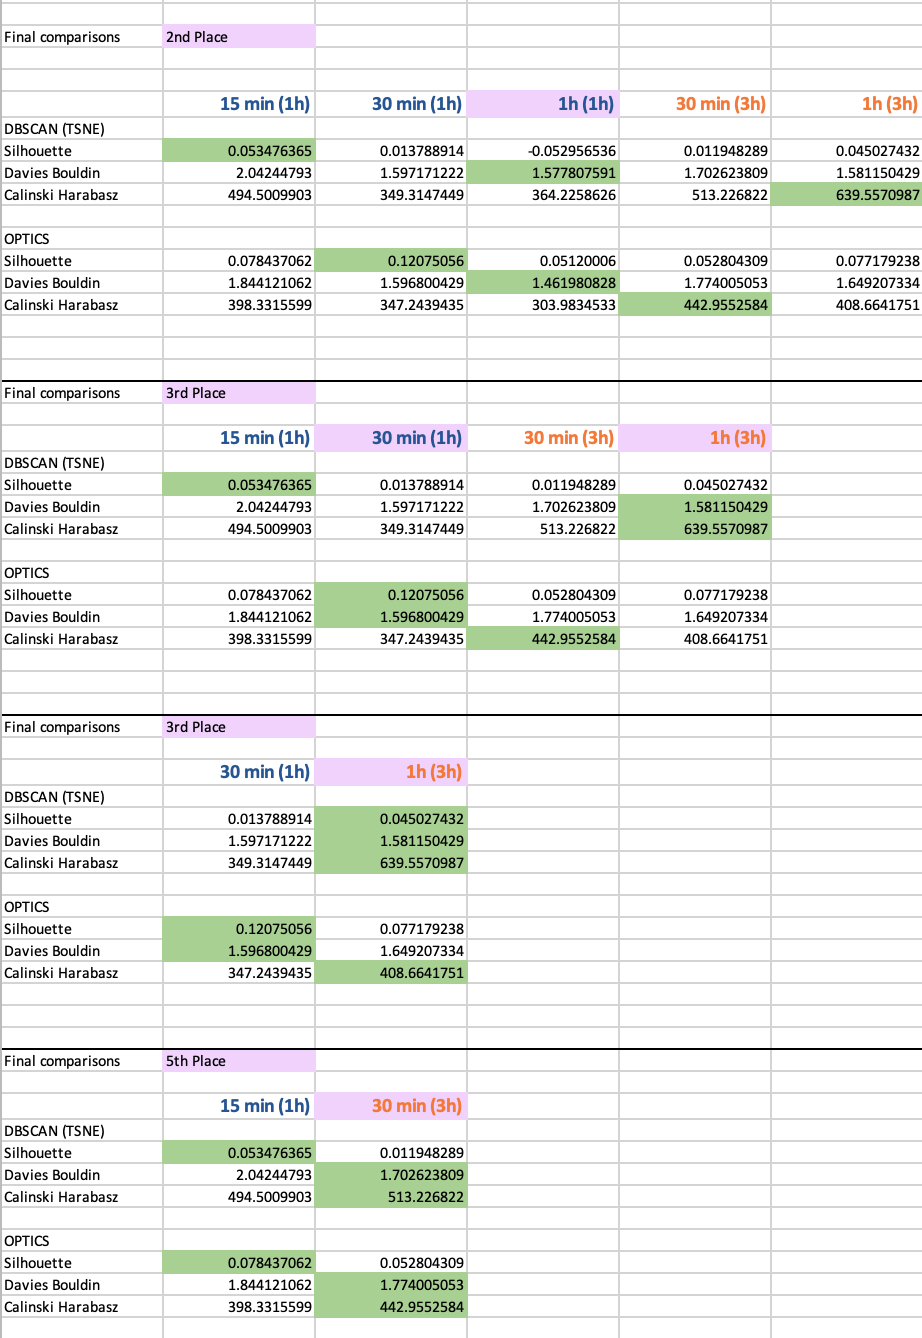
\includegraphics[width=0.8\textwidth]{./images/clusteringResults/clusteringResultsPlaces.png}
  \caption{Evaluation scores comparison to determine \textbf{2nd, 3rd, 4th, 5th, and 6th place}.}
  \label{figure:clusterResultsPlaces}
\end{figure}


\clearpage